\section{Introduction}

\DD{pomysl na intro: zdefiniowac dwa glowne problemy: learning + set cover; zapowiedziec, ze sa powiazane ze soba i celem papieru jest przestudiowanie tych zaleznosci plus usyskanie konkretnych wynikow; pytanie/do sprawdzenia: czy ktores wyniki przypadkiem poprawiaja lub sa tozsame z najlepszymi znanymi bez precedensow; ewentualne inna ``marketingowe'' uwagi.}

Consider a set $\cH$ of $n$ \emph{hypotheses}, a set $\cT$ of $m$ \emph{tests} and  an unknown \emph{target hypothesis} $\target\in\cH$ that needs to be discovered through an active learning process.
Each test $t\in\cT$ is a partition of $\cH$, that is, $t$ consists of subsets of $\cH$ such that $x\cap y=\emptyset$ for any $x,y\in t$ and $\bigcup t=\cH$.
As a result of executing a test $t\in\cT$, \questioner recives a \emph{reply} that reveals $x\in t$ such that $\target\in x$.
That is, the \questioner learns which subset of $\cH$ that belongs to $t$ contains the target.
Each subsequent test is selected by \questioner by taking into acocunt replies from all test to date.
Without formally stating an optimization criterion we refer to  the above as the \emph{Active Learing Process} ($\ProblemAL$).
(Another widely used name in the literature is the decision tree construction).
The goal for the \questioner is to output $\target$.

Consider an arbitrary partial order $(\cT,\preceq)$ that introduces a precedence relation between tests.
This leads us to the two active learning problems in which order to perform a test $t$, all its predecesors had to be performed previously.
Hence we have the \emph{Precedence Constrained Worst Case Active Learing} ($\ProblemPCWCAL$) in which the goal is to compute the $\ProblemAL$ that respects the precedence constraints and outputs the target $\target$ by performing the minimum number of tests in the worst case.
Similarly, in the \emph{Precedence Constrained Average Case Active Learing} ($\ProblemPCACAL$) the optimization criterion changes to minimizing the number of queries done on average.
Whenever the criterion is not important or we want to make a claim that applies to both we use the symbol $\ProblemPCAL$ to refer to a \emph{Precedence Constrained Active Learning} instance.


In this work we study connections between active lerning with precedences and the covering problems defined as follows.
We are given a set $\cU$ of $n$ items, a collection $\cS$ of $m$ subsets of $\cU$, such that $\bigcup\cS=\cU$, an arbitrary partial order $(\cS,\preceq)$ on these subsets and an integer $k$.
We say that a subfamily $\cC\subseteq\cS$ \emph{covers} at least $k$ items from $\cU$ if $\spr{\bigcup\cC}\geq k$.
We ask for a $\cC\subseteq\cS$ that covers at least $k$ items from $\cU$ and for each $x\in\cC$ and each $y\in\cS$ such that $y\preceq x$ it holds $y\in\cC$.
In the \emph{Precedence Constrained Set Cover} ($\ProblemPCSC$) the goal is to minimize $\spr{\cC}$.
A permutation $\br{C_1,\ldots,C_l}$ of the elements in $\cC$ is \emph{consistent} with the partial order $(\cS,\preceq)$ if for any $C_i$ and $C_j$ such that $C_i\preceq C_j$ it holds $i<j$.
The \emph{coverage time} of a $x\in\bigcup\cC$ is the minimum index $i$ such that $x\in C_i$.
In the \emph{Precedence Constrained Min-Sum Set Cover} ($\ProblemPCMSSC$) the goal is to find a sequence $(C_1,\ldots,C_k)$ that minimizes the total coverage time of all items in $C_1\cup\cdots\cup C_k$.


% Consider following problems:
% \begin{itemize}
%   \item  The \emph{Precedence Constrained Bayesian Active Learning Problem} consists a set of $\mathcal{H}$ of $n$ hypothesis, a set $\cT$ of $m$ tests and a DAG (directed acyclic graph) $\mathcal{F} = \brc{\cT, \preceq}$ encoding the precedence constraints between available tests. Among $\mathcal{H}$ a hidden hypothesis is required to be encovered. To do so, the learner is allowed to perform tests, each of which reveals partial information about the hidden hypothesis. Upon receiving this information, the learner actively selects the next test to be performed. Importantly, in order to perform such test the learner needs to perform all of its predecesors in $\mathcal{F}$ first. The goal is to uncover the hidden hypothesis while performing as few tests as possible. Depending on the chosen criterion we distinguish between the \emph{Precedence Constrained Worst Case Active Learning} (PCWCAL) and \emph{Precedence Constrained Average Case Active Learning} (PCACAL) problems.
%   \item The \emph{Precedence Constrained Covering Problem} consists of a set of $n$ items $\mathcal{U}$, a collection $\mathcal{S}$ of $m$ subsets of $\mathcal{U}$ that cover these items, and a DAG $\mathcal{F} = \brc{\mathcal{S}, \preceq}$ encoding the precedence constraints between available subsets. The goal is to select a sequence of tests that covers at least $K$ items. Depending on the chosen criterion we distinguish between the \emph{Precedence Constrained Set Cover} (PCSC) and \emph{Precedence Constrained Min-Sum Set Cover} (PCMSSC) problems. In the first we are only interested in minimizing the number of selected subsets, while in the second we want to minimize the average time it takes to cover an item.
% \end{itemize}

\subsection{Our results and techniques}

\DD{Pomysl na rozdzial:
\begin{itemize}
 \item zajawka, że wprpwadzimy nowe inne problemy (raz - jak pomocnicze; dwa - jako dopelnienie obrazu roznych rzeczy z litearatury)
 \item zdefiniowac pozostałe problemy z ``diagramu'' zaleznosci miedzy nimi
 \item diagram
 \item najwazniejsze twierdzenia
 \item tabelka na podsumowanie
\end{itemize}
}

Our main goal is to derive several complexity results regarding the problems introduced above.
Hence we start with stating the main results of this work.

\DD{Tutaj poszłyby główne twierdzenia dot. $\ProblemPCAL$, $\ProblemPCMSSC$ oraz $\ProblemPCSC$, czyli tych głównych z intro.}


\DD{Ten przykład jest super, ale chyba musimy znaleźć sposób na jego kompresję, tzn. nie stać nas na zapłacenie całej strony; około 1/3 strony byłaby ok (może tabelka obok drzewa decyzyjnego (moze zamiana kolumn vs wierszy aby ją powęzić, a może mocno zminimalizować przestrzeń między kolumnami, a partial order jako łuki pomiędzy etykietami wierszy tabelki?); też do przemyślenia gdzie ten przykład umieścić (raczej nie w ``contribution'', ale albo w intro, albo w preliminaries chyba}
\begin{figure}[htb!]
\centering
\centering

\begin{minipage}[t]{\textwidth}
\centering
\scalebox{0.76}{
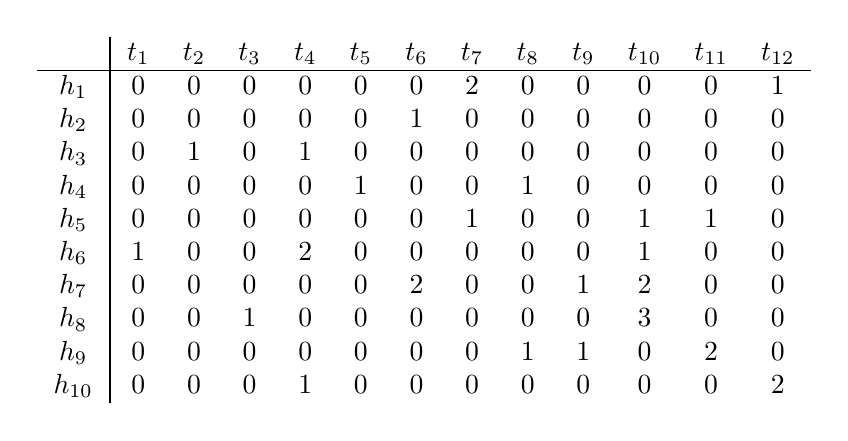
\begin{tikzpicture}[
    node distance=1cm,
    test/.style={circle, draw, thick, minimum size=0.6cm},
    decision/.style={circle, draw, thick, minimum size=0.55cm},
    leaf/.style={circle, draw, thick, fill=green!20, minimum size=0.5cm},
    arrow/.style={->, thick}
]

% Table of hypotheses vs tests (10 hypotheses, 12 tests, unbalanced outcomes)
\node[] at (0,0) {
\begin{tabular}{c|cccccccccccc}
 & $t_1$ & $t_2$ & $t_3$ & $t_4$ & $t_5$ & $t_6$ & $t_7$ & $t_8$ & $t_9$ & $t_{10}$ & $t_{11}$ & $t_{12}$ \\
\hline
$h_1$ & 0 & 0 & 0 & 0 & 0 & 0 & 2 & 0 & 0 & 0 & 0 & 1 \\
$h_2$ & 0 & 0 & 0 & 0 & 0 & 1 & 0 & 0 & 0 & 0 & 0 & 0 \\
$h_3$ & 0 & 1 & 0 & 1 & 0 & 0 & 0 & 0 & 0 & 0 & 0 & 0 \\
$h_4$ & 0 & 0 & 0 & 0 & 1 & 0 & 0 & 1 & 0 & 0 & 0 & 0 \\
$h_5$ & 0 & 0 & 0 & 0 & 0 & 0 & 1 & 0 & 0 & 1 & 1 & 0 \\
$h_6$ & 1 & 0 & 0 & 2 & 0 & 0 & 0 & 0 & 0 & 1 & 0 & 0 \\
$h_7$ & 0 & 0 & 0 & 0 & 0 & 2 & 0 & 0 & 1 & 2 & 0 & 0 \\
$h_8$ & 0 & 0 & 1 & 0 & 0 & 0 & 0 & 0 & 0 & 3 & 0 & 0 \\
$h_9$ & 0 & 0 & 0 & 0 & 0 & 0 & 0 & 1 & 1 & 0 & 2 & 0 \\
$h_{10}$ & 0 & 0 & 0 & 1 & 0 & 0 & 0 & 0 & 0 & 0 & 0 & 2 \\
\end{tabular}
};

\end{tikzpicture}
}
\normalsize
\caption*{(a) Hypotheses and tests table}
\end{minipage}

\begin{minipage}[t]{0.43\textwidth}
\centering
\scalebox{0.78}{
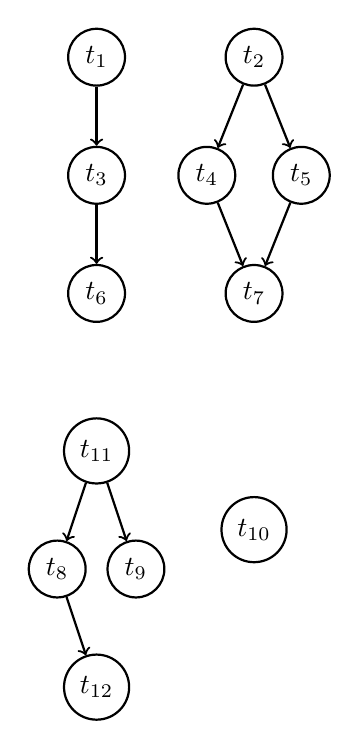
\begin{tikzpicture}[
    node distance=1cm,
    test/.style={circle, draw, thick, minimum size=0.6cm},
    arrow/.style={->, thick}
]

% DAG with 4 components (2 components on top, 2 below)
% Component 1 (top left)
\node[test] (t1) at (0.5,0) {$t_1$};
\node[test] (t3) at (0.5,-1.5) {$t_3$};
\node[test] (t6) at (0.5,-3) {$t_6$};
\draw[arrow] (t1) -- (t3);
\draw[arrow] (t3) -- (t6);

% Component 2 (top right)
\node[test] (t2) at (2.5,0) {$t_2$};
\node[test] (t4) at (1.9,-1.5) {$t_4$};
\node[test] (t5) at (3.1,-1.5) {$t_5$};
\node[test] (t7) at (2.5,-3) {$t_7$};
\draw[arrow] (t2) -- (t4);
\draw[arrow] (t2) -- (t5);
\draw[arrow] (t4) -- (t7);
\draw[arrow] (t5) -- (t7);

% Component 3 (bottom left)
\node[test] (t11) at (0.5,-5) {$t_{11}$};
\node[test] (t8) at (0,-6.5) {$t_8$};
\node[test] (t9) at (1,-6.5) {$t_9$};
\node[test] (t12) at (0.5,-8) {$t_{12}$};
\draw[arrow] (t11) -- (t8);
\draw[arrow] (t11) -- (t9);
\draw[arrow] (t8) -- (t12);

% Component 4 (isolated node, bottom right)
\node[test] (t10) at (2.5,-6) {$t_{10}$};

\end{tikzpicture}
}
\normalsize
\caption*{(b) Precedence}
\end{minipage}
\hfill
\begin{minipage}[t]{0.55\textwidth}
\centering
\scalebox{0.78}{
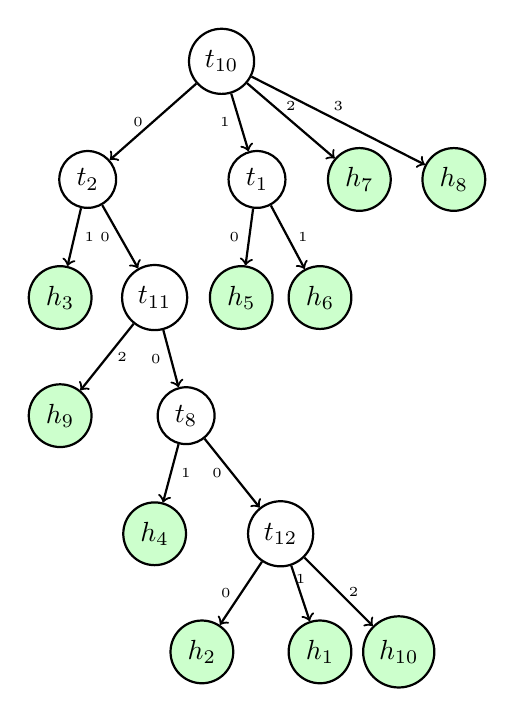
\begin{tikzpicture}[
    node distance=1cm,
    decision/.style={circle, draw, thick, minimum size=0.55cm},
    leaf/.style={circle, draw, thick, fill=green!20, minimum size=0.5cm},
    arrow/.style={->, thick}
]

% Decision tree built from table analysis
% Root: t10 (separates: h5→1, h6→1, h7→2, h8→3, rest→0)
\node[decision] (root) at (4.25,0) {$t_{10}$};

% t10=0: {h1,h2,h3,h4,h9,h10}
\node[decision] (n1) at (2.55,-1.5) {$t_2$};
% t10=1: {h5,h6}
\node[decision] (n2) at (4.7,-1.5) {$t_1$};
% t10=2: {h7}
\node[leaf] (h7) at (6,-1.5) {$h_7$};
% t10=3: {h8}
\node[leaf] (h8) at (7.2,-1.5) {$h_8$};

% t10=0, t2=0: {h1,h2,h4,h9,h10}
\node[decision] (n3) at (3.4,-3) {$t_{11}$};
% t10=0, t2=1: {h3}
\node[leaf] (h3) at (2.2,-3) {$h_3$};

% t10=1, t1=0: {h5}
\node[leaf] (h5) at (4.5,-3) {$h_5$};
% t10=1, t1=1: {h6}
\node[leaf] (h6) at (5.5,-3) {$h_6$};

% t10=0, t2=0, t11=0: {h1,h2,h4,h10}
\node[decision] (n4) at (3.8,-4.5) {$t_8$};
% t10=0, t2=0, t11=1: {h5} - but h5 already separated
% t10=0, t2=0, t11=2: {h9}
\node[leaf] (h9) at (2.2,-4.5) {$h_9$};

% t10=0, t2=0, t11=0, t8=0: {h1,h2,h10}
\node[decision] (n5) at (5,-6) {$t_{12}$};
% t10=0, t2=0, t11=0, t8=1: {h4}
\node[leaf] (h4) at (3.4,-6) {$h_4$};

% t10=0, t2=0, t11=0, t8=0, t12=0: {h2}
\node[leaf] (h2) at (4,-7.5) {$h_2$};
% t10=0, t2=0, t11=0, t8=0, t12=1: {h1}
\node[leaf] (h1) at (5.5,-7.5) {$h_1$};
% t10=0, t2=0, t11=0, t8=0, t12=2: {h10}
\node[leaf] (h10) at (6.5,-7.5) {$h_{10}$};

% Edges
\draw[arrow] (root) -- (n1) node[midway, left, font=\tiny] {0};
\draw[arrow] (root) -- (n2) node[midway, left, font=\tiny] {1};
\draw[arrow] (root) -- (h7) node[midway, above, font=\tiny] {2};
\draw[arrow] (root) -- (h8) node[midway, above, font=\tiny] {3};

\draw[arrow] (n1) -- (n3) node[midway, left, font=\tiny] {0};
\draw[arrow] (n1) -- (h3) node[midway, right, font=\tiny] {1};

\draw[arrow] (n2) -- (h5) node[midway, left, font=\tiny] {0};
\draw[arrow] (n2) -- (h6) node[midway, right, font=\tiny] {1};

\draw[arrow] (n3) -- (n4) node[midway, left, font=\tiny] {0};
\draw[arrow] (n3) -- (h9) node[midway, right, font=\tiny] {2};

\draw[arrow] (n4) -- (n5) node[midway, left, font=\tiny] {0};
\draw[arrow] (n4) -- (h4) node[midway, right, font=\tiny] {1};

\draw[arrow] (n5) -- (h2) node[midway, left, font=\tiny] {0};
\draw[arrow] (n5) -- (h1) node[midway, above, font=\tiny] {1};
\draw[arrow] (n5) -- (h10) node[midway, right, font=\tiny] {2};

\end{tikzpicture}
}
\normalsize
\caption*{(c) Valid decision tree}
\end{minipage}

\caption{Example of a $\ProblemPCAL$ instance with 10 hypotheses and 12 tests. (a) Hypotheses-tests table. (b) Precedence DAG with four components. (c) A valid decision tree solution respecting precedence constraints.}\label{fig:pcal_example}
\end{figure}

\DD{na razie zakomentowałem rysunek dot zbiorów}
% \begin{figure}[h]
% \centering
% \centering

\begin{minipage}[t]{0.6\textwidth}
\centering
\scalebox{0.57}{
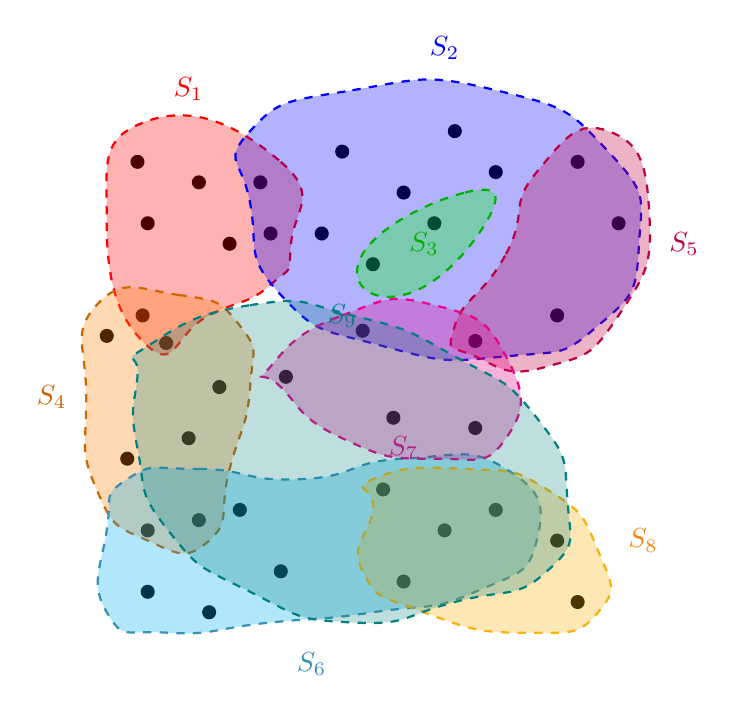
\begin{tikzpicture}[
    scale=1.3,
    node distance=1cm,
    element/.style={circle, draw, thick, fill=black, minimum size=0.15cm, inner sep=0pt},
    arrow/.style={->, thick}
]

% Universe elements - scattered randomly across the plane (35 elements with varied distribution)
\node[element] at (0.4, 3.9) {};
\node[element] at (0.9, 4.3) {};
\node[element] at (1.2, 3.7) {};
\node[element] at (0.35, 3) {};
\node[element] at (1.5, 4.3) {};
\node[element] at (0.3, 4.5) {};
\node[element] at (1.6, 3.8) {};  % SHARED by S1 and S2
\node[element] at (0.58, 2.73) {};  % SHARED by S1 and S4

\node[element] at (2.3, 4.6) {};
\node[element] at (2.9, 4.2) {};
\node[element] at (2.1, 3.8) {};
\node[element] at (3.4, 4.8) {};
\node[element] at (3.8, 4.4) {};
\node[element] at (2.6, 3.5) {};
\node[element] at (3.2, 3.9) {};

\node[element] at (4.6, 4.5) {};
\node[element] at (5, 3.9) {};
\node[element] at (4.4, 3) {};

\node[element] at (0, 2.8) {};
\node[element] at (1.1, 2.3) {};
\node[element] at (0.8, 1.8) {};
\node[element] at (0.2, 1.6) {};

\node[element] at (2.5, 2.85) {};
\node[element] at (3.6, 1.9) {};
\node[element] at (2.8, 2) {};
\node[element] at (3.6, 2.75) {};
\node[element] at (1.75, 2.4) {};

\node[element] at (0.9, 1.0) {};  % SHARED by S4 and S6
\node[element] at (0.4, 0.9) {};
\node[element] at (1.3, 1.1) {};
\node[element] at (0.4, 0.3) {};
\node[element] at (1.7, 0.5) {};
\node[element] at (1.0, 0.1) {};

\node[element] at (2.7, 1.3) {};
\node[element] at (3.3, 0.9) {};
\node[element] at (2.9, 0.4) {};
\node[element] at (3.8, 1.1) {};
\node[element] at (4.4, 0.8) {};
\node[element] at (4.6, 0.2) {};

% Set S1 (red) - includes (0.4,3.9) (0.9,4.3) (1.2,3.7) (0.6,3.2) (1.5,4.1) (0.3,4.5) + SHARED (1.6,4.0) (0.9,2.9)
\draw[thick, dashed, red, fill=red, fill opacity=0.3] 
    plot[smooth cycle, tension=1.0] coordinates {(0.4,4.9) (1.7,4.5) (1.8,3.7) (1.6,3.3) (1.0, 3) (0.4,2.7) (0.0,3.9)};
\node[above] at (0.8,5.0) {\textcolor{red}{$S_1$}};

% Set S2 (blue) - includes (2.3,4.6) (2.9,4.2) (2.1,3.8) (3.4,4.8) (3.8,4.4) (2.6,3.5) (3.2,3.9) (4.3,4.5) (4.7,3.9) (4.1,3.4) + SHARED (1.6,4.0)
\draw[thick, dashed, blue, fill=blue, fill opacity=0.3]
    plot[smooth cycle, tension=1.0] coordinates {(1.4,4.8) (2.4,5.2) (3.8,5.2) (4.9,4.6) (5.2,3.7) (4.8,2.9) (3.9,2.6) (2.7,2.7) (1.7,3.2) (1.4,4.1)};
\node[above] at (3.3,5.4) {\textcolor{blue}{$S_2$}};

% Set S3 (green) - small subset inside S2: (2.6,3.5) (3.2,3.9)
\draw[thick, dashed, green!70!black, fill=green, fill opacity=0.3]
    plot[smooth cycle, tension=1.0] coordinates {(2.5,3.6) (3.5,4.2) (3.7,3.9) (2.9,3.2)};
\node at (3.1,3.7) {\textcolor{green!70!black}{$S_3$}};

% Set S4 (orange) - includes (0.5,2.5) (1.1,2.8) (0.8,2.0) (0.2,1.6) + SHARED (0.9,1.0) (0.9,2.9)
\draw[thick, dashed, orange!80!black, fill=orange, fill opacity=0.3]
    plot[smooth cycle, tension=1.0] coordinates {(-0.1,3.1) (0.7,3.2) (1.3,2.9) (1.4,2.3) (1.2,1.5) (1.0,0.8) (0.4,0.8) (-0.1,1.3) (-0.2,2.2)};
\node[left] at (-0.3,2.2) {\textcolor{orange!80!black}{$S_4$}};

% Set S5 (purple) - right side elongated: (3.6,2.6) overlaps with S2 for (4.3,4.5) (4.7,3.9) (4.1,3.4)
\draw[thick, dashed, purple, fill=purple, fill opacity=0.3]
    plot[smooth cycle, tension=1.0] coordinates {(3.4,2.9) (3.9,3.6) (4.2,4.4) (4.9,4.8) (5.3,4.0) (5.0,3.0) (4.3,2.5) (3.6,2.6)};
\node[right] at (5.4,3.7) {\textcolor{purple}{$S_5$}};

% Set S6 (cyan) - includes (0.9,1.0) (0.7,0.8) (1.3,1.1) (0.4,0.3) (1.7,0.5) (1.0,0.1) (2.7,1.3) (3.3,0.9) (2.9,0.4) (3.8,1.1)
\draw[thick, dashed, cyan!70!black, fill=cyan, fill opacity=0.3]
    plot[smooth cycle, tension=1.0] coordinates {(0.2,1.4) (0.9,1.5) (1.9,1.4) (2.9,1.6) (3.9,1.5) (4.2,0.8) (3.6,0.3) (2.6,0.1) (1.6,0.0) (0.6,-0.1) (0.0,0.1) (0.0,0.9)};
\node[below] at (2.0,-0.2) {\textcolor{cyan!70!black}{$S_6$}};

% Set S7 (magenta) - includes (2.5,2.9) (3.1,2.4) (2.8,1.9) (1.9,2.2)
\draw[thick, dashed, magenta, fill=magenta, fill opacity=0.3]
    plot[smooth cycle, tension=1.0] coordinates {(1.6,2.5) (2.3,3.0) (3.2,3.1) (3.9,2.6) (3.9,1.8) (3.2,1.6) (2.3,1.8) (1.7,2.3)};
\node[above] at (2.9,1.5) {\textcolor{magenta}{$S_7$}};

% Set S8 (yellow!70!red) - includes (3.8,1.1) (4.4,0.6) (3.3,0.9) (2.9,0.4)
\draw[thick, dashed, yellow!70!red, fill=yellow!70!red, fill opacity=0.3]
    plot[smooth cycle, tension=1.0] coordinates {(2.6,1.4) (3.5,1.5) (4.3,1.3) (4.8,0.7) (4.8,0.1) (4.1,-0.1) (3.1,0.1) (2.5,0.5) (2.6,1.1)};
\node[right] at (5.0,0.8) {\textcolor{yellow!50!red}{$S_8$}};

% Set S9 (teal) - large blob filling gaps: overlaps with others to ensure complete coverage
\draw[thick, dashed, teal, fill=teal, fill opacity=0.25]
    plot[smooth cycle, tension=1.0] coordinates {(0.4,2.7) (1.4,3.1) (2.4,3.0) (3.4,2.6) (4.2,2.0) (4.5,1.2) (4.3,0.5) (3.4,0.2) (2.4,0.0) (1.4,0.3) (0.6,0.9) (0.3,1.7) (0.3,2.4)};
\node[below] at (2.3,3.2) {\textcolor{teal}{$S_9$}};

\end{tikzpicture}
}
\normalsize
\caption*{(a) Universe and sets}
\end{minipage}
\hfill
\begin{minipage}[t]{0.35\textwidth}
\centering
\scalebox{0.57}{
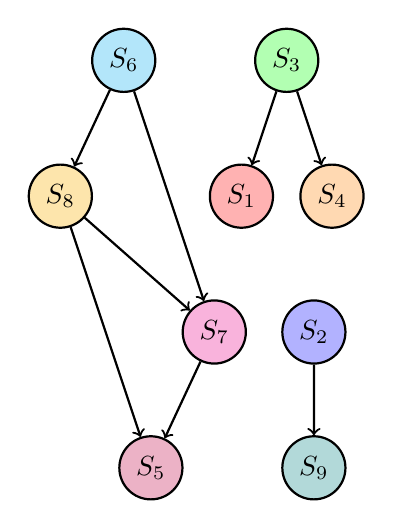
\begin{tikzpicture}[
    scale=1.15,
    node distance=1cm,
    set/.style={circle, draw, thick, minimum size=0.65cm},
    arrow/.style={->, thick}
]

% Precedence DAG with specified precedence constraints

% Component with S6 (left, wider)
\node[set, fill=cyan!30] (s6) at (0,0) {$S_6$};
\node[set, fill=yellow!70!red!30] (s8) at (-0.7,-1.5) {$S_8$};
\node[set, fill=magenta!30] (s7) at (1,-3) {$S_7$};
\node[set, fill=purple!30] (s5) at (0.3,-4.5) {$S_5$};

% Component with S3 (right top)
\node[set, fill=green!30] (s3) at (1.8,0) {$S_3$};
\node[set, fill=red!30] (s1) at (1.3,-1.5) {$S_1$};
\node[set, fill=orange!30] (s4) at (2.3,-1.5) {$S_4$};

% Component with S2 (right bottom)
\node[set, fill=blue!30] (s2) at (2.1,-3) {$S_2$};
\node[set, fill=teal!30] (s9) at (2.1,-4.5) {$S_9$};

% Precedence constraints (all arrows go down)
\draw[arrow] (s3) -- (s1);
\draw[arrow] (s3) -- (s4);
\draw[arrow] (s6) -- (s7);
\draw[arrow] (s6) -- (s8);
\draw[arrow] (s8) -- (s7);
\draw[arrow] (s8) -- (s5);
\draw[arrow] (s7) -- (s5);
\draw[arrow] (s2) -- (s9);

\end{tikzpicture}
}
\normalsize
\caption*{(b) Precedence}
\end{minipage}

\vspace{0.5cm}

\begin{minipage}[t]{\textwidth}
\centering
\scalebox{0.765}{
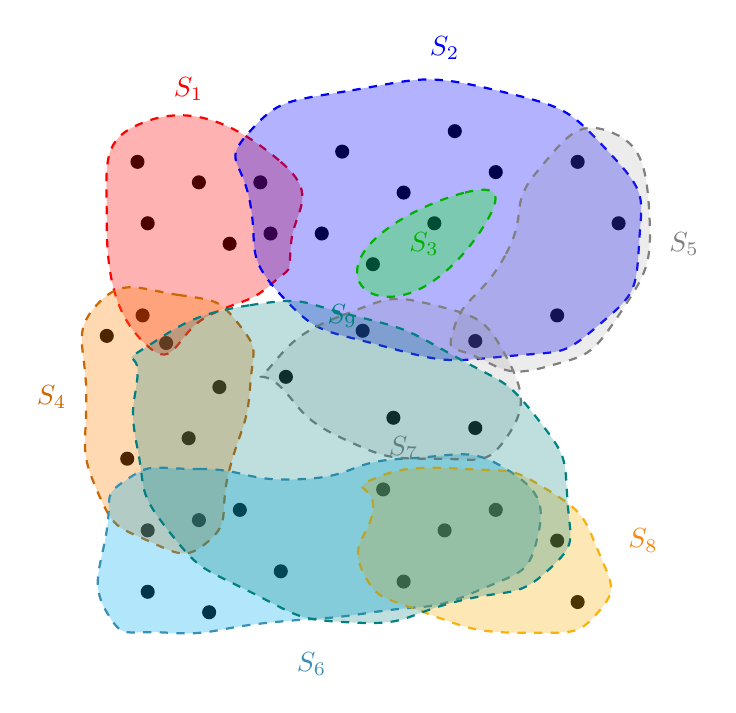
\begin{tikzpicture}[
    scale=1.3,
    node distance=1cm,
    element/.style={circle, draw, thick, fill=black, minimum size=0.15cm, inner sep=0pt},
    arrow/.style={->, thick}
]

% Universe elements - scattered randomly across the plane (35 elements with varied distribution)
\node[element] at (0.4, 3.9) {};
\node[element] at (0.9, 4.3) {};
\node[element] at (1.2, 3.7) {};
\node[element] at (0.35, 3) {};
\node[element] at (1.5, 4.3) {};
\node[element] at (0.3, 4.5) {};
\node[element] at (1.6, 3.8) {};  % SHARED by S1 and S2
\node[element] at (0.58, 2.73) {};  % SHARED by S1 and S4

\node[element] at (2.3, 4.6) {};
\node[element] at (2.9, 4.2) {};
\node[element] at (2.1, 3.8) {};
\node[element] at (3.4, 4.8) {};
\node[element] at (3.8, 4.4) {};
\node[element] at (2.6, 3.5) {};
\node[element] at (3.2, 3.9) {};

\node[element] at (4.6, 4.5) {};
\node[element] at (5, 3.9) {};
\node[element] at (4.4, 3) {};

\node[element] at (0, 2.8) {};
\node[element] at (1.1, 2.3) {};
\node[element] at (0.8, 1.8) {};
\node[element] at (0.2, 1.6) {};

\node[element] at (2.5, 2.85) {};
\node[element] at (3.6, 1.9) {};
\node[element] at (2.8, 2) {};
\node[element] at (3.6, 2.75) {};
\node[element] at (1.75, 2.4) {};

\node[element] at (0.9, 1.0) {};  % SHARED by S4 and S6
\node[element] at (0.4, 0.9) {};
\node[element] at (1.3, 1.1) {};
\node[element] at (0.4, 0.3) {};
\node[element] at (1.7, 0.5) {};
\node[element] at (1.0, 0.1) {};

\node[element] at (2.7, 1.3) {};
\node[element] at (3.3, 0.9) {};
\node[element] at (2.9, 0.4) {};
\node[element] at (3.8, 1.1) {};
\node[element] at (4.4, 0.8) {};
\node[element] at (4.6, 0.2) {};

% Set S1 (red) - SELECTED
\draw[thick, dashed, red, fill=red, fill opacity=0.3] 
    plot[smooth cycle, tension=1.0] coordinates {(0.4,4.9) (1.7,4.5) (1.8,3.7) (1.6,3.3) (1.0, 3) (0.4,2.7) (0.0,3.9)};
\node[above] at (0.8,5.0) {\textcolor{red}{\textbf{$S_1$}}};

% Set S2 (blue) - SELECTED
\draw[thick, dashed, blue, fill=blue, fill opacity=0.3]
    plot[smooth cycle, tension=1.0] coordinates {(1.4,4.8) (2.4,5.2) (3.8,5.2) (4.9,4.6) (5.2,3.7) (4.8,2.9) (3.9,2.6) (2.7,2.7) (1.7,3.2) (1.4,4.1)};
\node[above] at (3.3,5.4) {\textcolor{blue}{\textbf{$S_2$}}};

% Set S3 (green) - SELECTED
\draw[thick, dashed, green!70!black, fill=green, fill opacity=0.3]
    plot[smooth cycle, tension=1.0] coordinates {(2.5,3.6) (3.5,4.2) (3.7,3.9) (2.9,3.2)};
\node at (3.1,3.7) {\textcolor{green!70!black}{\textbf{$S_3$}}};

% Set S4 (orange) - SELECTED
\draw[thick, dashed, orange!80!black, fill=orange, fill opacity=0.3]
    plot[smooth cycle, tension=1.0] coordinates {(-0.1,3.1) (0.7,3.2) (1.3,2.9) (1.4,2.3) (1.2,1.5) (1.0,0.8) (0.4,0.8) (-0.1,1.3) (-0.2,2.2)};
\node[left] at (-0.3,2.2) {\textcolor{orange!80!black}{\textbf{$S_4$}}};

% Set S5 (purple) - NOT SELECTED (grayed out)
\draw[thick, dashed, gray, fill=gray, fill opacity=0.15]
    plot[smooth cycle, tension=1.0] coordinates {(3.4,2.9) (3.9,3.6) (4.2,4.4) (4.9,4.8) (5.3,4.0) (5.0,3.0) (4.3,2.5) (3.6,2.6)};
\node[right] at (5.4,3.7) {\textcolor{gray}{$S_5$}};

% Set S6 (cyan) - SELECTED
\draw[thick, dashed, cyan!70!black, fill=cyan, fill opacity=0.3]
    plot[smooth cycle, tension=1.0] coordinates {(0.2,1.4) (0.9,1.5) (1.9,1.4) (2.9,1.6) (3.9,1.5) (4.2,0.8) (3.6,0.3) (2.6,0.1) (1.6,0.0) (0.6,-0.1) (0.0,0.1) (0.0,0.9)};
\node[below] at (2.0,-0.2) {\textcolor{cyan!70!black}{\textbf{$S_6$}}};

% Set S7 (magenta) - NOT SELECTED (grayed out)
\draw[thick, dashed, gray, fill=gray, fill opacity=0.15]
    plot[smooth cycle, tension=1.0] coordinates {(1.6,2.5) (2.3,3.0) (3.2,3.1) (3.9,2.6) (3.9,1.8) (3.2,1.6) (2.3,1.8) (1.7,2.3)};
\node[above] at (2.9,1.5) {\textcolor{gray}{$S_7$}};

% Set S8 (yellow!70!red) - SELECTED
\draw[thick, dashed, yellow!70!red, fill=yellow!70!red, fill opacity=0.3]
    plot[smooth cycle, tension=1.0] coordinates {(2.6,1.4) (3.5,1.5) (4.3,1.3) (4.8,0.7) (4.8,0.1) (4.1,-0.1) (3.1,0.1) (2.5,0.5) (2.6,1.1)};
\node[right] at (5.0,0.8) {\textcolor{yellow!50!red}{\textbf{$S_8$}}};

% Set S9 (teal) - SELECTED
\draw[thick, dashed, teal, fill=teal, fill opacity=0.25]
    plot[smooth cycle, tension=1.0] coordinates {(0.4,2.7) (1.4,3.1) (2.4,3.0) (3.4,2.6) (4.2,2.0) (4.5,1.2) (4.3,0.5) (3.4,0.2) (2.4,0.0) (1.4,0.3) (0.6,0.9) (0.3,1.7) (0.3,2.4)};
\node[below] at (2.3,3.2) {\textcolor{teal}{\textbf{$S_9$}}};

\end{tikzpicture}
}
\normalsize
\caption*{(c) Solution: $\{S_1, S_2, S_6, S_8, S_9\}$ (in color)}
\end{minipage}


% \caption{Example of a PCCP instance with 39 elements and 9 covering sets. (a) Universe with covering sets. (b) Precedence DAG with three components. (c) Solution using 7 selected sets (colored).}\label{fig:pccp_example}
% \end{figure}

Our main results are obtained through several algorithmic ``reductions'' by which we mean that we use approximation algorithms for selected problems to obtain approximations for others.
In order to show a full picture of our method we introduce three remaining problems that paly an important role in our approach.

\begin{definition}[Group Steiner Tree (GST)]
Given an undirected graph $G = (V, E)$ with edge costs, a root vertex $r \in V$, and groups $g_1, \ldots, g_k \subseteq V$, find a minimum-cost tree $T$ rooted at $r$ that contains at least one vertex from each group $g_i$.
\end{definition}

\begin{definition}[Precedence constrained test cover (PCTC)]
Given a set $\cH$ of $n$ hypotheses, a set $\cT$ of $m$ tests, and a partial order $\brc{\cT, \preceq}$ encoding precedence constraints for $\cT$, find a precedence-closed subfamily of tests that distinguishes all pairs of hypotheses.
\end{definition}
\DD{czyli taka inna nazwa na test cover zaaplikowany bezposrednio do hipotez?}

% \begin{figure}[h]
% \centering
% \centering

\begin{minipage}[t]{0.6\textwidth}
\centering
\scalebox{0.57}{
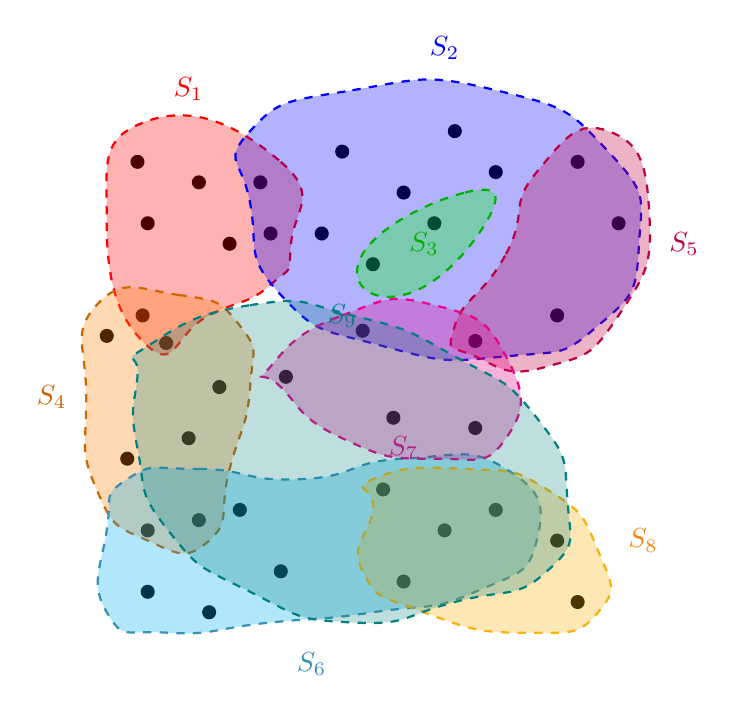
\begin{tikzpicture}[
    scale=1.3,
    node distance=1cm,
    element/.style={circle, draw, thick, fill=black, minimum size=0.15cm, inner sep=0pt},
    arrow/.style={->, thick}
]

% Universe elements - scattered randomly across the plane (35 elements with varied distribution)
\node[element] at (0.4, 3.9) {};
\node[element] at (0.9, 4.3) {};
\node[element] at (1.2, 3.7) {};
\node[element] at (0.35, 3) {};
\node[element] at (1.5, 4.3) {};
\node[element] at (0.3, 4.5) {};
\node[element] at (1.6, 3.8) {};  % SHARED by S1 and S2
\node[element] at (0.58, 2.73) {};  % SHARED by S1 and S4

\node[element] at (2.3, 4.6) {};
\node[element] at (2.9, 4.2) {};
\node[element] at (2.1, 3.8) {};
\node[element] at (3.4, 4.8) {};
\node[element] at (3.8, 4.4) {};
\node[element] at (2.6, 3.5) {};
\node[element] at (3.2, 3.9) {};

\node[element] at (4.6, 4.5) {};
\node[element] at (5, 3.9) {};
\node[element] at (4.4, 3) {};

\node[element] at (0, 2.8) {};
\node[element] at (1.1, 2.3) {};
\node[element] at (0.8, 1.8) {};
\node[element] at (0.2, 1.6) {};

\node[element] at (2.5, 2.85) {};
\node[element] at (3.6, 1.9) {};
\node[element] at (2.8, 2) {};
\node[element] at (3.6, 2.75) {};
\node[element] at (1.75, 2.4) {};

\node[element] at (0.9, 1.0) {};  % SHARED by S4 and S6
\node[element] at (0.4, 0.9) {};
\node[element] at (1.3, 1.1) {};
\node[element] at (0.4, 0.3) {};
\node[element] at (1.7, 0.5) {};
\node[element] at (1.0, 0.1) {};

\node[element] at (2.7, 1.3) {};
\node[element] at (3.3, 0.9) {};
\node[element] at (2.9, 0.4) {};
\node[element] at (3.8, 1.1) {};
\node[element] at (4.4, 0.8) {};
\node[element] at (4.6, 0.2) {};

% Set S1 (red) - includes (0.4,3.9) (0.9,4.3) (1.2,3.7) (0.6,3.2) (1.5,4.1) (0.3,4.5) + SHARED (1.6,4.0) (0.9,2.9)
\draw[thick, dashed, red, fill=red, fill opacity=0.3] 
    plot[smooth cycle, tension=1.0] coordinates {(0.4,4.9) (1.7,4.5) (1.8,3.7) (1.6,3.3) (1.0, 3) (0.4,2.7) (0.0,3.9)};
\node[above] at (0.8,5.0) {\textcolor{red}{$S_1$}};

% Set S2 (blue) - includes (2.3,4.6) (2.9,4.2) (2.1,3.8) (3.4,4.8) (3.8,4.4) (2.6,3.5) (3.2,3.9) (4.3,4.5) (4.7,3.9) (4.1,3.4) + SHARED (1.6,4.0)
\draw[thick, dashed, blue, fill=blue, fill opacity=0.3]
    plot[smooth cycle, tension=1.0] coordinates {(1.4,4.8) (2.4,5.2) (3.8,5.2) (4.9,4.6) (5.2,3.7) (4.8,2.9) (3.9,2.6) (2.7,2.7) (1.7,3.2) (1.4,4.1)};
\node[above] at (3.3,5.4) {\textcolor{blue}{$S_2$}};

% Set S3 (green) - small subset inside S2: (2.6,3.5) (3.2,3.9)
\draw[thick, dashed, green!70!black, fill=green, fill opacity=0.3]
    plot[smooth cycle, tension=1.0] coordinates {(2.5,3.6) (3.5,4.2) (3.7,3.9) (2.9,3.2)};
\node at (3.1,3.7) {\textcolor{green!70!black}{$S_3$}};

% Set S4 (orange) - includes (0.5,2.5) (1.1,2.8) (0.8,2.0) (0.2,1.6) + SHARED (0.9,1.0) (0.9,2.9)
\draw[thick, dashed, orange!80!black, fill=orange, fill opacity=0.3]
    plot[smooth cycle, tension=1.0] coordinates {(-0.1,3.1) (0.7,3.2) (1.3,2.9) (1.4,2.3) (1.2,1.5) (1.0,0.8) (0.4,0.8) (-0.1,1.3) (-0.2,2.2)};
\node[left] at (-0.3,2.2) {\textcolor{orange!80!black}{$S_4$}};

% Set S5 (purple) - right side elongated: (3.6,2.6) overlaps with S2 for (4.3,4.5) (4.7,3.9) (4.1,3.4)
\draw[thick, dashed, purple, fill=purple, fill opacity=0.3]
    plot[smooth cycle, tension=1.0] coordinates {(3.4,2.9) (3.9,3.6) (4.2,4.4) (4.9,4.8) (5.3,4.0) (5.0,3.0) (4.3,2.5) (3.6,2.6)};
\node[right] at (5.4,3.7) {\textcolor{purple}{$S_5$}};

% Set S6 (cyan) - includes (0.9,1.0) (0.7,0.8) (1.3,1.1) (0.4,0.3) (1.7,0.5) (1.0,0.1) (2.7,1.3) (3.3,0.9) (2.9,0.4) (3.8,1.1)
\draw[thick, dashed, cyan!70!black, fill=cyan, fill opacity=0.3]
    plot[smooth cycle, tension=1.0] coordinates {(0.2,1.4) (0.9,1.5) (1.9,1.4) (2.9,1.6) (3.9,1.5) (4.2,0.8) (3.6,0.3) (2.6,0.1) (1.6,0.0) (0.6,-0.1) (0.0,0.1) (0.0,0.9)};
\node[below] at (2.0,-0.2) {\textcolor{cyan!70!black}{$S_6$}};

% Set S7 (magenta) - includes (2.5,2.9) (3.1,2.4) (2.8,1.9) (1.9,2.2)
\draw[thick, dashed, magenta, fill=magenta, fill opacity=0.3]
    plot[smooth cycle, tension=1.0] coordinates {(1.6,2.5) (2.3,3.0) (3.2,3.1) (3.9,2.6) (3.9,1.8) (3.2,1.6) (2.3,1.8) (1.7,2.3)};
\node[above] at (2.9,1.5) {\textcolor{magenta}{$S_7$}};

% Set S8 (yellow!70!red) - includes (3.8,1.1) (4.4,0.6) (3.3,0.9) (2.9,0.4)
\draw[thick, dashed, yellow!70!red, fill=yellow!70!red, fill opacity=0.3]
    plot[smooth cycle, tension=1.0] coordinates {(2.6,1.4) (3.5,1.5) (4.3,1.3) (4.8,0.7) (4.8,0.1) (4.1,-0.1) (3.1,0.1) (2.5,0.5) (2.6,1.1)};
\node[right] at (5.0,0.8) {\textcolor{yellow!50!red}{$S_8$}};

% Set S9 (teal) - large blob filling gaps: overlaps with others to ensure complete coverage
\draw[thick, dashed, teal, fill=teal, fill opacity=0.25]
    plot[smooth cycle, tension=1.0] coordinates {(0.4,2.7) (1.4,3.1) (2.4,3.0) (3.4,2.6) (4.2,2.0) (4.5,1.2) (4.3,0.5) (3.4,0.2) (2.4,0.0) (1.4,0.3) (0.6,0.9) (0.3,1.7) (0.3,2.4)};
\node[below] at (2.3,3.2) {\textcolor{teal}{$S_9$}};

\end{tikzpicture}
}
\normalsize
\caption*{(a) Universe and sets}
\end{minipage}
\hfill
\begin{minipage}[t]{0.35\textwidth}
\centering
\scalebox{0.57}{
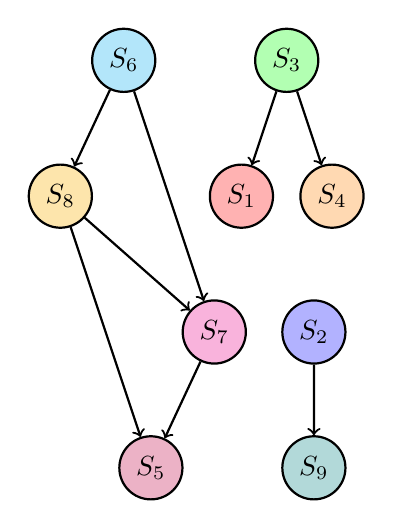
\begin{tikzpicture}[
    scale=1.15,
    node distance=1cm,
    set/.style={circle, draw, thick, minimum size=0.65cm},
    arrow/.style={->, thick}
]

% Precedence DAG with specified precedence constraints

% Component with S6 (left, wider)
\node[set, fill=cyan!30] (s6) at (0,0) {$S_6$};
\node[set, fill=yellow!70!red!30] (s8) at (-0.7,-1.5) {$S_8$};
\node[set, fill=magenta!30] (s7) at (1,-3) {$S_7$};
\node[set, fill=purple!30] (s5) at (0.3,-4.5) {$S_5$};

% Component with S3 (right top)
\node[set, fill=green!30] (s3) at (1.8,0) {$S_3$};
\node[set, fill=red!30] (s1) at (1.3,-1.5) {$S_1$};
\node[set, fill=orange!30] (s4) at (2.3,-1.5) {$S_4$};

% Component with S2 (right bottom)
\node[set, fill=blue!30] (s2) at (2.1,-3) {$S_2$};
\node[set, fill=teal!30] (s9) at (2.1,-4.5) {$S_9$};

% Precedence constraints (all arrows go down)
\draw[arrow] (s3) -- (s1);
\draw[arrow] (s3) -- (s4);
\draw[arrow] (s6) -- (s7);
\draw[arrow] (s6) -- (s8);
\draw[arrow] (s8) -- (s7);
\draw[arrow] (s8) -- (s5);
\draw[arrow] (s7) -- (s5);
\draw[arrow] (s2) -- (s9);

\end{tikzpicture}
}
\normalsize
\caption*{(b) Precedence}
\end{minipage}

\vspace{0.5cm}

\begin{minipage}[t]{\textwidth}
\centering
\scalebox{0.765}{
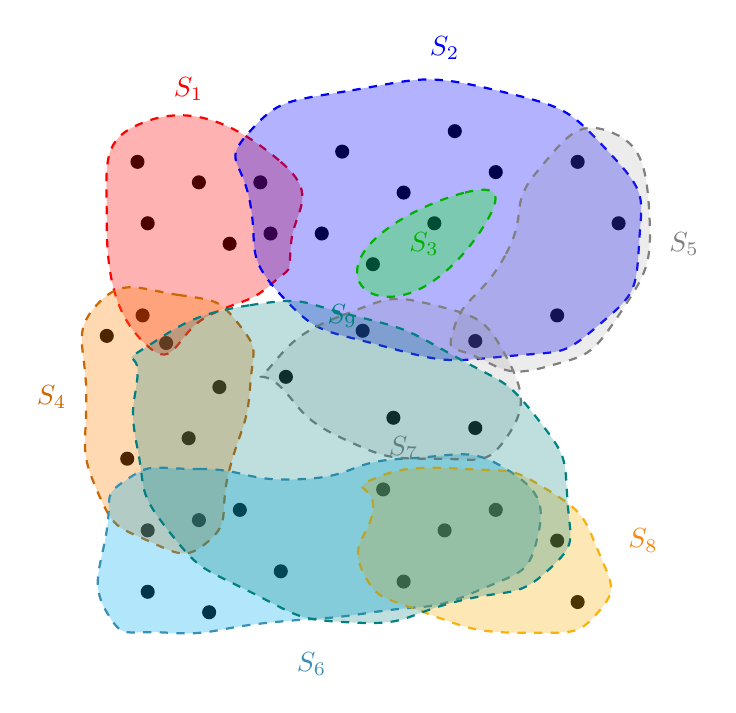
\begin{tikzpicture}[
    scale=1.3,
    node distance=1cm,
    element/.style={circle, draw, thick, fill=black, minimum size=0.15cm, inner sep=0pt},
    arrow/.style={->, thick}
]

% Universe elements - scattered randomly across the plane (35 elements with varied distribution)
\node[element] at (0.4, 3.9) {};
\node[element] at (0.9, 4.3) {};
\node[element] at (1.2, 3.7) {};
\node[element] at (0.35, 3) {};
\node[element] at (1.5, 4.3) {};
\node[element] at (0.3, 4.5) {};
\node[element] at (1.6, 3.8) {};  % SHARED by S1 and S2
\node[element] at (0.58, 2.73) {};  % SHARED by S1 and S4

\node[element] at (2.3, 4.6) {};
\node[element] at (2.9, 4.2) {};
\node[element] at (2.1, 3.8) {};
\node[element] at (3.4, 4.8) {};
\node[element] at (3.8, 4.4) {};
\node[element] at (2.6, 3.5) {};
\node[element] at (3.2, 3.9) {};

\node[element] at (4.6, 4.5) {};
\node[element] at (5, 3.9) {};
\node[element] at (4.4, 3) {};

\node[element] at (0, 2.8) {};
\node[element] at (1.1, 2.3) {};
\node[element] at (0.8, 1.8) {};
\node[element] at (0.2, 1.6) {};

\node[element] at (2.5, 2.85) {};
\node[element] at (3.6, 1.9) {};
\node[element] at (2.8, 2) {};
\node[element] at (3.6, 2.75) {};
\node[element] at (1.75, 2.4) {};

\node[element] at (0.9, 1.0) {};  % SHARED by S4 and S6
\node[element] at (0.4, 0.9) {};
\node[element] at (1.3, 1.1) {};
\node[element] at (0.4, 0.3) {};
\node[element] at (1.7, 0.5) {};
\node[element] at (1.0, 0.1) {};

\node[element] at (2.7, 1.3) {};
\node[element] at (3.3, 0.9) {};
\node[element] at (2.9, 0.4) {};
\node[element] at (3.8, 1.1) {};
\node[element] at (4.4, 0.8) {};
\node[element] at (4.6, 0.2) {};

% Set S1 (red) - SELECTED
\draw[thick, dashed, red, fill=red, fill opacity=0.3] 
    plot[smooth cycle, tension=1.0] coordinates {(0.4,4.9) (1.7,4.5) (1.8,3.7) (1.6,3.3) (1.0, 3) (0.4,2.7) (0.0,3.9)};
\node[above] at (0.8,5.0) {\textcolor{red}{\textbf{$S_1$}}};

% Set S2 (blue) - SELECTED
\draw[thick, dashed, blue, fill=blue, fill opacity=0.3]
    plot[smooth cycle, tension=1.0] coordinates {(1.4,4.8) (2.4,5.2) (3.8,5.2) (4.9,4.6) (5.2,3.7) (4.8,2.9) (3.9,2.6) (2.7,2.7) (1.7,3.2) (1.4,4.1)};
\node[above] at (3.3,5.4) {\textcolor{blue}{\textbf{$S_2$}}};

% Set S3 (green) - SELECTED
\draw[thick, dashed, green!70!black, fill=green, fill opacity=0.3]
    plot[smooth cycle, tension=1.0] coordinates {(2.5,3.6) (3.5,4.2) (3.7,3.9) (2.9,3.2)};
\node at (3.1,3.7) {\textcolor{green!70!black}{\textbf{$S_3$}}};

% Set S4 (orange) - SELECTED
\draw[thick, dashed, orange!80!black, fill=orange, fill opacity=0.3]
    plot[smooth cycle, tension=1.0] coordinates {(-0.1,3.1) (0.7,3.2) (1.3,2.9) (1.4,2.3) (1.2,1.5) (1.0,0.8) (0.4,0.8) (-0.1,1.3) (-0.2,2.2)};
\node[left] at (-0.3,2.2) {\textcolor{orange!80!black}{\textbf{$S_4$}}};

% Set S5 (purple) - NOT SELECTED (grayed out)
\draw[thick, dashed, gray, fill=gray, fill opacity=0.15]
    plot[smooth cycle, tension=1.0] coordinates {(3.4,2.9) (3.9,3.6) (4.2,4.4) (4.9,4.8) (5.3,4.0) (5.0,3.0) (4.3,2.5) (3.6,2.6)};
\node[right] at (5.4,3.7) {\textcolor{gray}{$S_5$}};

% Set S6 (cyan) - SELECTED
\draw[thick, dashed, cyan!70!black, fill=cyan, fill opacity=0.3]
    plot[smooth cycle, tension=1.0] coordinates {(0.2,1.4) (0.9,1.5) (1.9,1.4) (2.9,1.6) (3.9,1.5) (4.2,0.8) (3.6,0.3) (2.6,0.1) (1.6,0.0) (0.6,-0.1) (0.0,0.1) (0.0,0.9)};
\node[below] at (2.0,-0.2) {\textcolor{cyan!70!black}{\textbf{$S_6$}}};

% Set S7 (magenta) - NOT SELECTED (grayed out)
\draw[thick, dashed, gray, fill=gray, fill opacity=0.15]
    plot[smooth cycle, tension=1.0] coordinates {(1.6,2.5) (2.3,3.0) (3.2,3.1) (3.9,2.6) (3.9,1.8) (3.2,1.6) (2.3,1.8) (1.7,2.3)};
\node[above] at (2.9,1.5) {\textcolor{gray}{$S_7$}};

% Set S8 (yellow!70!red) - SELECTED
\draw[thick, dashed, yellow!70!red, fill=yellow!70!red, fill opacity=0.3]
    plot[smooth cycle, tension=1.0] coordinates {(2.6,1.4) (3.5,1.5) (4.3,1.3) (4.8,0.7) (4.8,0.1) (4.1,-0.1) (3.1,0.1) (2.5,0.5) (2.6,1.1)};
\node[right] at (5.0,0.8) {\textcolor{yellow!50!red}{\textbf{$S_8$}}};

% Set S9 (teal) - SELECTED
\draw[thick, dashed, teal, fill=teal, fill opacity=0.25]
    plot[smooth cycle, tension=1.0] coordinates {(0.4,2.7) (1.4,3.1) (2.4,3.0) (3.4,2.6) (4.2,2.0) (4.5,1.2) (4.3,0.5) (3.4,0.2) (2.4,0.0) (1.4,0.3) (0.6,0.9) (0.3,1.7) (0.3,2.4)};
\node[below] at (2.3,3.2) {\textcolor{teal}{\textbf{$S_9$}}};

\end{tikzpicture}
}
\normalsize
\caption*{(c) Solution: $\{S_1, S_2, S_6, S_8, S_9\}$ (in color)}
\end{minipage}


% \caption{Example of a PCCP instance with 39 elements and 9 covering sets. (a) Universe with covering sets. (b) Precedence DAG with three components. (c) Solution using 7 selected sets (colored).}\label{fig:pccp_example}
% \end{figure}


\begin{table}[htb!]
\centering
\begin{tabular}{|l|c|c|c|c|}
\hline
\textbf{precedence/problem} & \textbf{PCSC} & \textbf{PCMSSC} & \textbf{PCWCAL} & \textbf{PCACAL} \\
\hline
none & $O(\log n)$ & 4 & $O(\log n)$ & $O(\log n)$ \\
% \hline
% paths & $O(\log n)$* & 4 & $O(\log n)$* & $O(\log n)$* \\
\hline
inforest & $O(\log n)$* & 4 & $O(\log n)$* & $O(\log n)$* \\
\hline
outforest & $O(\log^2 n)$** & $O(\log n)$** & $O(\log^2 n)$* & $O(\log^2 n)$* \\
\hline
general & $O(\sqrt{m}\log n)$* & $O(\sqrt{m})$ & $O(\sqrt{m}\log n)$* & $O(\sqrt{m}\log n)$* \\
\hline
\end{tabular}
\caption{Approximation algorithms for various covering and active learning problems under different precedence constraints. (* denotes new results, ** denotes previously unmentioned corollaries of known results).}\label{tab:results}
\end{table}

\begin{figure}[h]
\centering
\begin{tikzpicture}[
    node distance=2.5cm and 3cm,
    problem/.style={rectangle, draw, very thick, minimum width=2.2cm, minimum height=1cm, align=center, font=\small},
    arrow/.style={->, very thick}
]

% Third row (define first for positioning)
\node[problem] (pcmssc) {PCMSSC};
\node[problem, right=3cm of pcmssc] (pcsc) {PCSC};

% Second row (above pcsc)
\node[problem, above right=0.7cm and 2cm of pcsc] (gst) {GST};

% Top row (above gst)
\node[problem, above left=0.6cm and 1.5cm of gst] (mdpcs) {MDPCS};

% Bottom row
\node[problem, below=0.6cm of pcmssc] (pcacal) {PCACAL};
\node[problem, below=0.6cm of pcsc] (pcwcal) {PCWCAL};
\node[problem, right=3cm of pcwcal] (pctc) {PCTC};

% Arrows
\draw[arrow] (mdpcs) -- (gst);
\draw[arrow] (mdpcs) -- (pcsc);
\draw[arrow] (mdpcs) -- (pcmssc);
\draw[arrow] (gst) -- (pcsc);
\draw[arrow] (pcsc) -- (pctc);
\draw[arrow] (pcsc) -- (pcwcal);
\draw[arrow] (pcmssc) -- (pcacal);

\end{tikzpicture}

\caption{Relationships between covering and active learning problems, $\Pi_1 \to \Pi_2$ denotes that an approximation algorithm for problem $\Pi_1$ implies an approximation algorithm for problem $\Pi_2$.}\label{fig:reductions}
\end{figure}

